\documentclass[11pt]{article}
\usepackage[margin=1in]{geometry}
\usepackage{float}
\usepackage{xcolor}

\usepackage{wrapfig}
\usepackage{subcaption}
\usepackage{caption}

\usepackage{amsmath, amsthm, amssymb, mathtools}
\usepackage{newpxtext, newpxmath}

\usepackage{physics}

\NewDocumentCommand{\R}{}{\mathbb{R}}

\usepackage{thmtools}

\RenewDocumentCommand{\qedsymbol}{}{$\blacksquare$}

\declaretheorem{theorem}
\declaretheorem{lemma}
\declaretheorem[style=definition]{definition}

\declaretheorem[style=remark]{example}
\declaretheorem[style=remark]{remark}

\usepackage{tikz}
\usetikzlibrary{arrows}
\usetikzlibrary{arrows.meta}

\usepackage[style=alphabetic]{biblatex}
\addbibresource{sources/library.bib}

\tikzset{
    vertex/.style={
        font = \scriptsize,
        fill=blue!20,
        draw,
        circle,
        inner sep=0pt,
        minimum size=20pt,
    },
    edge/.style={}
}

\NewDocumentCommand{\term}{m}{\emph{#1}}
\NewDocumentCommand{\thh}{}{\text{th}}

\usepackage{hyperref}

\hypersetup{
    colorlinks,
    citecolor=blue,
    linkcolor=blue,
    filecolor=blue,      
    urlcolor=blue,
}

\title{The Graph Laplacian and Determining the Connectivity of Meshes}
\author{Eli Griffiths}
\date{November 2024}

\directlua{graph = require("graph")}
\directlua{examples = require("data")}

\begin{document}

\maketitle

\begin{abstract}
    Graphs lend themselves naturally to matrices that encode properties such as which vertices are connected to others and how many vertices are connected to a given vertex. These matrix representations allow us to analyze graphs outside of traditional combinatoric approaches by considering their eigenvalues and eigenvectors. Key to our study is the Laplacian matrix representation of a graph. We first show that the eigenvalues of the Laplacian matrix give insight into if every vertex of a graph is connected to each other via some path through edges, and if not how many separate components there are in which this is the case. We then frame this result within the context of of computational geometry and discuss how more advanced problems in computational geometry can be approached with this spectral framework.
\end{abstract}

\section{Introduction}

Graphs at their core encode connectivity. A graph is simply vertices and edges where vertices are objects and edges are connections between these objects. While simple in concept, this means that anywhere there are pairwise relationships between objects, a graph structure can be assigned. We see graphs appear in situations such as modeling friendship networks on social media platform, determining flight schedules for optimal transport, modeling the structure of chemical compounds, and of importance to us computational geometry. Because of the fundamental nature of connectivity in many differing fields and applications, it is of great interest to develop theories and algorithms for graphs.

Graph theory as a field has always been deeply tied to combinatorics. One of the earliest problems in graph theory is Euler's famous K\"onigsberg bridge problem. In the town of K\"onigsberg, there were $7$ bridges connecting $4$ land masses. The question is if if there was a possible route one could walk that would cross each bridge exactly once. Euler reframed the problem by considering the bridges as edges and each land mass as vertices. By employing the fundamental concept of counting from combinatorics, Euler solved the problem in terms of the parity of the number of edges going into a vertex for each land mass \cite{wilson2013combinatorics}. %TODO: Make connection to modern graph theory

In this paper, we will explore an alternative way of viewing and understanding graphs. We will seek to construct a bridge between the discrete graph structure and a more algebraic description. The question is what algebraic description or structure should we use? Note that if we limit the number of vertices of a graph to be finite, we can index its vertices as $v_1, \ldots, v_n$. We can then lay out in a $2$D grid all possible pairs of vertices and mark each cell when the corresponding vertices are connected. Quite naturally, this same grid could be expressed as a matrix where each row and column represents some vertex and the entries are $1$ if two vertices are connected and $0$ otherwise. We will find that such possible matrix representations of graphs will have well behaved spectra (that is well behaved eigenvalues and eigenvectors). We will then show that the connectedness of a graph is encoded in the eigenvalues of a certain matrix representation of a graph, a result we can then reframe in computational geometry.

\section{Background}

We first outline the formal structure of a graph and related definitions that will be used throughout the paper, following the formalism and notation from \cite{diestelGraphTheory2017}. We denote $[S]^n$ as the set of all $n$-element sized subsets of $S$.

\begin{definition}[Graph Structure]
    A \term{graph} is a pair $G = (V, E)$ of sets where $E \subseteq [V]^2$. The elements of $V$ are \term{vertices} and the elements of $E$ are \term{edges}. A vertex $v$ is said to be \term{incident} to an edge $e$ if $v \in e$. Two vertices $v_1$ and $v_2$ are \term{adjacent} or \term{neighbors} if $\qty{v_1, v_2} \in E$. We denote $\qty{v_1, v_2} \in E$ by $v_1 \sim v_2$. The \term{set of neighbors} of a vertex $v$ is denoted by $N(v) \coloneq \qty{w \in V : v \sim w}$. The \term{degree} of a vertex $v$ is $\deg(v) \coloneq |N(v)|$. A \term{subgraph} $H$ of $G$, denoted by $H \subseteq G$, is a graph whose vertex and edge sets are subsets of $G$'s.
\end{definition}

\begin{remark}
    Edges importantly are defined here as two element sets and not as ordered pairs. This makes the graph \textit{undirected}.
\end{remark}

\begin{figure}
    \centering
    \begin{subfigure}[t]{0.45\textwidth}
        \centering
        \begin{tikzpicture}[scale=0.8]
            \directlua{graph.graph_tikz(examples.example1)}
        \end{tikzpicture}   
        \caption{A graph with $7$ vertices and $15$ edges}
        \label{fig:basic_graph}
    \end{subfigure}\hfill
    \begin{subfigure}[t]{0.45\textwidth}
        \centering
        \begin{tikzpicture}[scale=0.8]
            \directlua{graph.graph_tikz(examples.example2)}
        \end{tikzpicture}   
        \caption{A graph with $2$ connected components}
        \label{fig:connected_components}
    \end{subfigure}
    \caption{Two example graphs in the plane}
    \label{fig:graph_visual}
\end{figure}

For the purposes of this paper, we will assume that every graph has finitely many vertices (and hence finitely many edges). Consider the illustrations of two graphs in Figure \ref{fig:graph_visual}. Notice that they differ in terms of how connected their vertices are to one other. If each vertex was a city and each edge a road, a car driving on \ref{fig:basic_graph} could get to any city, but a car on the outer ring of \ref{fig:connected_components} would be stuck on the outer ring. That is, there is some path that the car can take from any city to any other city in \ref{fig:basic_graph} but not in \ref{fig:connected_components}. We formalize this notion of paths and connectedness as follows.

\begin{definition}[Connectedness]
    A \term{path} is a non-empty graph $P = (V,E)$ where
    \[
        V = \qty{v_0, v_1, \ldots, v_k} \hspace{2cm} E = \qty{\qty{v_0,v_1}, \ldots, \qty{v_{k-1}, v_k}}
    .\]
    A graph $G$ is then \term{connected} if between any two vertices $v_0$ and $v_f$ there exists a path $P \subseteq G$ starting at $v_0$ and ending at $v_f$. A \term{connected component} of a graph is a subgraph $H \subseteq G$ that is connected and is not contained in any larger connected subgraph.
\end{definition}

% \begin{remark}
%     Every graph has at least one connected component
% \end{remark}

\begin{example}
    Consider the graphs in Figure \ref{fig:graph_visual}. A possible path in \ref{fig:basic_graph} is $\qty{v_5, v_2, v_7, v_3}$ which means that $v_5$ and $v_3$ are connected. In \ref{fig:connected_components}, the subgraphs $\qty{v_1, \ldots, v_7}$ and $\qty{v_8, \ldots, v_{14}}$ are both connected components.
\end{example}

As previously discussed we will attempt to gain insight about graphs, and specifically their connectivity, by representing them algebraically as matrices. Of importance to us are the adjacency matrix and degree matrix which both capture in different ways the connectivity between vertices.

\begin{definition}
    The \term{adjacency matrix} $A_G$ and \term{degree matrix} $D_G$ of a graph $G$ with $n$ vertices are the $n \times n$ matrices such that
    \begin{align*}
        (A_G)_{ij} = \begin{cases}
            1 & v_i \sim v_j \\
            0 & \text{otherwise}
        \end{cases} & &
        (D_G)_{ij} = \begin{cases}
            \deg(v_i) & i = j \\
            0 & i \neq j
        \end{cases}
    \end{align*}
    If $G$ is understood via context, we simply refer to them as $A$ and $D$.
\end{definition}

\begin{example}
    \label{ex:adj_deg_mats}
    The adjacency and degree matrices for the graph in Figure \ref{fig:basic_graph} are

    \begin{align*}
        A =    
        \begin{bmatrix}
            \directlua{graph.adj_matrix(examples.example1)}
        \end{bmatrix} & &
        D = \begin{bmatrix}
            \directlua{graph.deg_matrix(examples.example1)}
        \end{bmatrix}
    \end{align*}
\end{example}

By observation, we can see that both the matrices in Example \ref{ex:adj_deg_mats} are symmetric matrices. One may recall from linear algebra important results about symmetric matrices and their spectra. Symmetric matrices are guaranteed to have real eigenvalues, an orthonormal basis of eigenvectors that diagonalize them, and many other properties. Generally speaking then, the spectra of a symmetric matrix is well behaved and numerically friendly. This begs the question of $(1)$ are the adjacency and degree matrices always symmetric for any graph, and $(2)$ if they are symmetric what insight could we possibly ascertain from their spectra? It turns out the answer to the first question is yes (as the next theorem demonstrates) and we will attempt to answer the second question in the next two sections.

\begin{theorem}
    \label{thm:adj_deg_symmetric}
    The adjacency and degree matrices $A$ and $D$ of a graph $G$ are symmetric.
\end{theorem}

\begin{proof}
    By the definition of the degree matrix, the only non zero entries lie on the main diagonal of $D$. Therefore $D$ is a diagonal matrix and hence symmetric. Consider two vertices $v_i, v_j$ of $G$ in which $v_i \sim v_j$. Since the edges of $G$ are undirected we also have $v_j \sim v_i$. Hence $(A)_{ij} = (A)_{ji} = 1$. Likewise, if $v_i \not\sim v_j$ then $v_j \not\sim v_i$ meaning $(A)_{ij} = (A)_{ji} = 0$. Therefore $A$ is symmetric.
\end{proof}

\section{A Graph's Spectra}

\begin{definition}
    The \term{Laplacian Matrix} of a graph $G$ is $L_G \coloneq D_G - A_G$. If $G$ is understood via context, we simply refer to it as $L$.
\end{definition}

Notice that since $L$ is the difference of two symmetric matrices it is also symmetric. Therefore we know that it has eigenvalues that are all real. Of importance to us is that amongst these eigenvalues, we are guaranteed to have zero as an eigenvalue for any Laplacian matrix.

\begin{theorem}
    \label{thm:lap_zero_eig_always}
    The Laplacian matrix $L$ of a graph $G$ has zero as an eigenvalue.
\end{theorem}

\begin{proof}
    Let $n$ denote the number of vertices in $G$ and take $x \in \R^n$ to be the vector of all $1$'s. By the definition of the Laplacian matrix, we have $L = D - A$. Consider the product $D x$. Since $D$ is diagonal, the $i^\thh$ component will be the $i^\thh$ component of $x$ times the $i^\thh$ entry along the diagonal of $D$, which by the definition of $D$ gives $(Dx)_i = \deg v_i$. Now consider the $i^\thh$ component of the product $Ax$. We can express it as the sum
    \[
        (Ax)_i = \sum_{j=1}^n (A)_{ij} x_j = \sum_{j=1}^n (A_{ij})
    .\]
    This sum is simply adding up the entries of the $i^\thh$ row of $A$. Since the entries are only $0$ and $1$, and are only $1$ when $v_i$ is adjacent to another vertex, the sum is $\deg v_i$. Hence $(Ax)_i = \deg v_i$. Thus $Ax = Dx$ from which we have $Lx = (D - A)x = Dx - Ax = 0$. Therefore zero is an eigenvalue of $L$.
\end{proof}

We will find in further analysis more utility in an alternative description of the Laplacian matrix. If we assign a real number to each vertex of a graph with $n$ vertices, we can view this as a vector in $x \in \R^n$ where each component corresponds to a vertex. Therefore the Laplacian matrix can be used to in a sense operate on $x$ like in $Lx$. This gives rise to the \emph{quadratic form} of the Laplacian. We will not provide a derivation of it here, but one can be found in \cite{mohar2004graph}.

\begin{theorem}
    Let $L$ be the Laplacian matrix of a finite graph $G$ with $n$ vertices. Then for a given vector $x \in \R^n$,
    \[
        x^T L x = \sum_{v_i \sim v_j} (x_i - x_j)^2.
    \]
\end{theorem}

\begin{remark}
    Sometimes the Laplacian matrix is defined as the unique symmetric matrix $L$ with this quadratic form and the matrix definition is then a derived representation \cite{WATKINS199443}. The quadratic form also helps motivate the choice to name $L$ the Laplacian matrix. In continuous settings, the Laplacian operator $\nabla$ ``smooths'' functions and averages locally large differences. In the matrix case, if we viewed a vector $x \in \R^n$ as a list of temperatures at each vertex of a graph, minimizing the quadratic form of its Laplacian matrix would act to diffuse heat in a smooth manner that like wise would average locally large differences.
\end{remark}

We are almost equipped with what we need to draw the connection between the Laplacian matrix's spectra and the connectivity of its corresponding graph. The following result about block diagonal matrices and their determinant will be needed, but we shall omit the proof of it here. A proof of this result can be found in \cite{silvester2000determinants}.

\begin{lemma}
    \label{lem:block_det}
    For a block diagonal matrix $A$ with blocks $A_i$, $\det(A) = \det(A_1) \det(A_2) \cdots \det(A_n)$
\end{lemma}

The following lemma gives a very strict characterization of zero as an eigenvalue for connected graphs. We will then generalize this characterization from a connected graph to any graph $G$ by decomposing it into its connected components.

\begin{lemma}
    \label{lem:eig0_iff_connected}
    A graph $G$ is connected if and only if the algebraic multiplicity of zero is $1$ for $L_G$.
\end{lemma}

\begin{proof}
    We proceed with the contrapositive of the reverse direction. Suppose that $G$ is not connected. If $k$ is the number of connected components of $G$ then $k > 1$. Denote each connected component as $H_i$. Note that each components vertex set must be pairwise disjoint with any other component then itself. Therefore we can group the vertices of $G$ by which subgraph $H_i$ they are in. If we then consider the adjacency matrix $A$ of $G$ with such an ordering, we will have a block diagonal matrix where each block is the adjacency matrix $A_i$ corresponding to each $H_i$. Thus the Laplacian matrix for $G$ is also block diagonal with each block being the Laplacian matrix $L_i$ for each $H_i$. Consider the characteristic polynomial $\det(L - I\lambda)$ of $L$. Since $L$ is block diagonal, by Lemma \ref{lem:block_det} we can expand this as $\det(L - I\lambda) = \det(L_1 - I\lambda) \cdots \det(L_k - I \lambda)$. For each $L_i$ we know from Lemma \ref{thm:lap_zero_eig_always} that each $L_i$ has zero as an eigenvalue and hence has the linear factor $(\lambda-0)$ in its characteristic polynomial. Therefore $\det(L - I\lambda)$ is the product of at least two terms that both have $(\lambda-0)$ as a factor, hence the multiplicity of zero for $L$ is greater than $1$.

    Suppose towards contradiction that $G$ is connected but the algebraic multiplicity of zero is not equal to $1$. Then the algebraic multiplicity of zero must be greater than $1$. Therefore the associated eigenspace must have a dimension greater than $1$, meaning we can pick two linearly independent eigenvectors $u$ and $w$. Since both are eigenvectors with eigenvalue $0$, we have
    \[
        \sum_{v_i \sim v_j} (u_i - u_j)^2 = u^T L u = u^T \mathbf{0} = 0
    \]
    which is true for $w$ as well. Since the quadratic form is a sum of non-negative terms, the only way it is zero is if every term is itself $0$. Therefore if $v_i \sim v_j$ we have $u_i = u_j$ and $w_i = w_j$. Consider two vertices $v_m$ and $v_n$ of $G$. Since $G$ is connected, there must exist a path between them. Note then that $u_m = u_n$ and $w_m = w_n$ since the equality of each component holds across each edge in the path. But since we can choose any two arbitrary vertices $v_m$ and $v_n$, every component of $u$ and $w$ are just constants. However, this means both $u$ and $w$ are scalar multiples of the vector of all $1$'s and hence are linearly dependent, a contradiction.
\end{proof}

\begin{theorem}
    \label{thm:main_thm}
    A graph $G$ has $m$ connected components if and only if the algebraic multiplicity of zero is $m$ for $L_G$.
\end{theorem}

\begin{proof}
    Suppose $G$ has $m$ connected components. Then the Laplacian matrix $L$ can be expressed as a block diagonal matrix since both the adjacency and degree matrix can be expressed as block diagonal. Each block $L_i$ represents the corresponding Laplacian matrix for the subgraph induced by each component. From Lemma \ref{lem:block_det}, we then have $\det(L - I \lambda) = \det(L_1 - I \lambda) \cdots \det(L_m - I \lambda)$ meaning the algebraic multiplicity of zero for $L$ is the sum of the algebraic multiplicities of zero for each $L_i$. Each $L_i$ is connected so by Lemma \ref{lem:eig0_iff_connected} we know the algebraic multiplicity of zero for each $L_i$ is one. Therefore the algebraic multiplicity of zero for $L$ is one summed up $m$ times which is just $m$. Now suppose the algebraic multiplicity of $L$ is $m$. Since $G$ is finite, we can let $k$ denote the number of connected components of $G$. By the same logic as above, $k$ must be the sum of the algebraic multiplicities of $0$ for each component. But this sum is simply $m$ meaning $k = m$.
\end{proof}

\section{Application to Computational Geometry}

\captionsetup{justification=centering,singlelinecheck=false}
\begin{wrapfigure}[6]{r}{0.25\textwidth}
    \vspace{-2.1cm}
    \begin{center}
        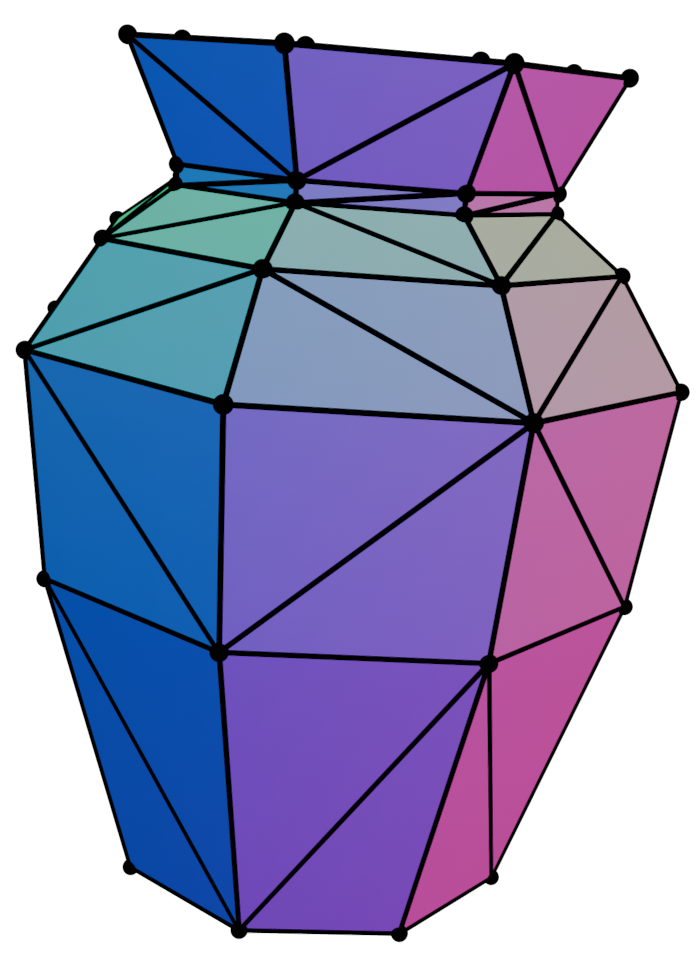
\includegraphics[width=0.20\textwidth]{figures/vase_all_cropped.png}
    \end{center}
    \caption{An example mesh}
    \label{fig:vase}
\end{wrapfigure}


In computer graphics, modeling, simulation, etc. we often want a representation of some real world geometry that we can perform computations on. A common way to of doing so is via a mesh. Consider the example mesh of a vase to the right. From some basic observations, the mesh appears to be comprised of points connected by segments/edges which outline faces. We formalize these observations in Definition \ref{def:tri_mesh}.

\begin{definition}
    \label{def:tri_mesh}
    A \term{triangular mesh} is a triple $K = (V, E, F)$ such that
    \begin{itemize}
        \item $V \subseteq \R^3$ is a finite set representing the vertices
        \item $E \subseteq [V]^2$ is a set representing edges
        \item $F \subseteq [E]^3$ is a set representing faces such that for any $f = \qty{e_1, e_2, e_3} \in F$, 
            \[
                e_1 \cap e_2 = \qty{v_1} \hspace{1cm} e_2 \cap e_3 = \qty{v_2} \hspace{1cm} e_3 \cap e_1 = \qty{v_3}
            .\]
            for $v_1 \neq v_2 \neq v_3$ and there are no three faces $f_1, f_2, f_3 \in F$ such that $f_1 \cap f_2 \cap f_3 = \qty{e}$.
    \end{itemize}
\end{definition}

\begin{wrapfigure}[13]{r}{0.25\textwidth}
    \vspace{-0.60cm}
    \begin{center}
        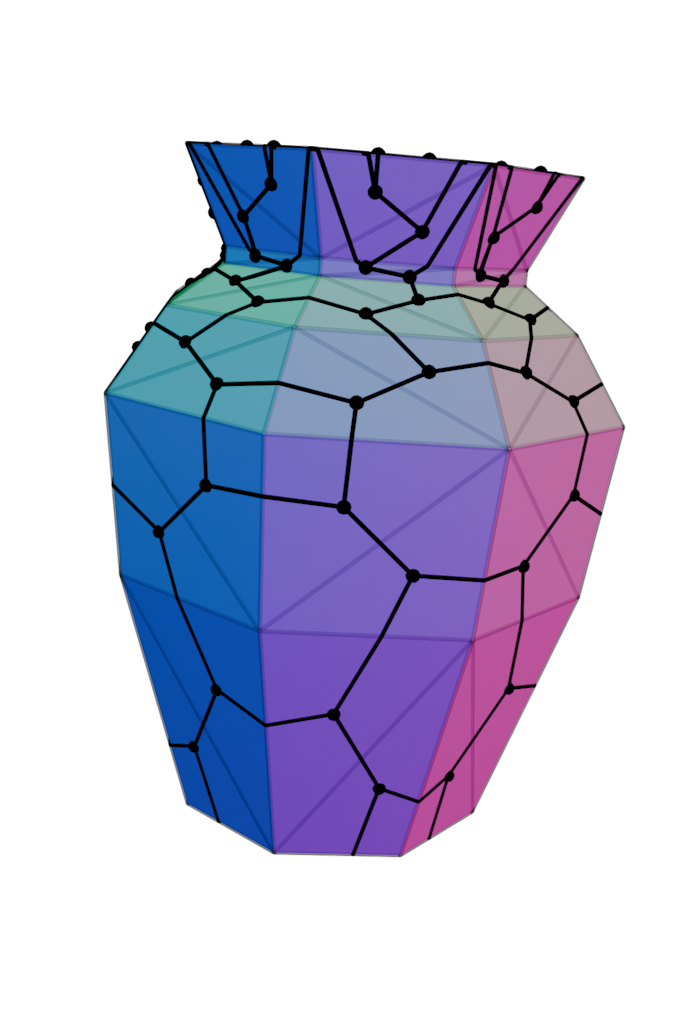
\includegraphics[width=0.20\textwidth]{figures/vase_dual.png}
    \end{center}
    \caption{\\
        Dual mesh of Fig. \ref{fig:vase}}
    \label{fig:vase_dual}
\end{wrapfigure}

Notice that a triangular mesh lends itself to some very natural graph structures. One is simply using the vertices as the graph vertices and the edges as graph edges. The other one which is of use to us is using the faces as graph vertices and faces sharing a common edge as the edge set. This is often referred to as the dual graph of a mesh and appears in computational geometry problems such as mesh based signal processing \cite{taubinDualMeshResampling2002} and refinement of meshed implicit surfaces \cite{10.1145/566282.566308}. 

\begin{definition}
    The \term{dual mesh} of a triangular mesh $K = (V_K, E_K, F_K)$ is the graph $G = (V, E)$ such that $V = F_K$ and $f_1 \sim f_2$ if $f_1 \cap f_2 = \qty{e}$ for some in $e \in E_K$.
\end{definition}

\begin{example}
    We can superimpose the dual mesh visually on the vase mesh in Figure \ref{fig:vase} by placing vertices on each face and connecting them on the surface of the vase itself, which can be seen in Figure \ref{fig:vase_dual}.
\end{example}

When dealing with meshes, we are usually interested in capturing the surface geometry of some object. It is very natural to ask questions about traversing or simulating heat dispersion on the surface of a mesh. Both of these tasks necessitate some concept of when parts of the mesh are connected to ensure paths don't jump between different unconnected parts or heat spreads through empty space. 

Imagine living on the surface of some face of a mesh. Then you can freely walk around the surface of that face. Furthermore, you can walk across edges to adjacent faces in well defined manner as there can only be at most $1$ possible choice due to the last restriction on faces in Definition \ref{def:tri_mesh}. Passing through a vertex is less well defined because there can be an arbitrary number of possible faces to go to.

We will therefore define (quite informally) that a mesh is \term{connected} if for any two points (starting on faces) can be connected via a path on the mesh surface that crosses between faces via edges only. In the same vain as a graph, a \term{connected component} of a mesh is a maximal submesh that is connected. This quickly lends itself to a reframing of Theorem \ref{thm:main_thm}.

\begin{theorem}
    A triangular mesh has $m$ connected components if and only if the algebraic multiplicity of zero is $m$ Laplacian matrix of its dual mesh has algebraic multiplicity $k$.
\end{theorem}

\begin{proof}
    The notion of connectedness for meshes we constructed is captured by the connectivity of the dual mesh. Our requirement that mesh connectivity happen across edges only is identical to connecting faces with a common edge as in the definition of the dual mesh. Therefore the question of how many connected components a mesh has is the same as how many connected components does its dual mesh have. Its dual mesh will have a corresponding Laplacian matrix which we know from Theorem \ref{thm:main_thm} that the algebraic multiplicity of zero equals the number of connected components. Therefore since the number of connected components in the mesh is identical to the number of connected components of its dual mesh, we have the desired if and only if.
\end{proof}

While this result may seem obvious having seen it established in a graph theory context, it serves to illustrate how simple it can be to translate results from graph theory to computational geometry. If one wanted to, they could use the previous result and find the multiplicity of a meshes zero eigenvalue numerically to determine how many components it has. This general approach we took of taking the dual, creating the Laplacian matrix of the dual, then applying some result about its spectra lends itself to some very powerful algorithms. While we were interested in a strict sense of connectivity, one may wonder if the connectivity of a graph could be represented as a more continuous quantity. This question lends itself to the realm of \term{spectral partitioning} in which a (possibly already connected mesh) is separated into submeshes that maximize some more continuous sense of connectedness. This separation is typically dictated by examining the unit norm eigenvector associated with the next largest eigenvalue than zero of the Laplacian matrix (called the ``Fiedler Vector''). Spectral partitioning gives very natural groupings of a mesh making it useful in medical applications \cite{10.1007/978-3-642-15705-9_41} and mesh processing \cite{bao2023spectral} (see Figure \ref{fig:spectral_part}).

\begin{figure}
    \centering
    \begin{subfigure}[t]{0.5\textwidth}
        \centering
        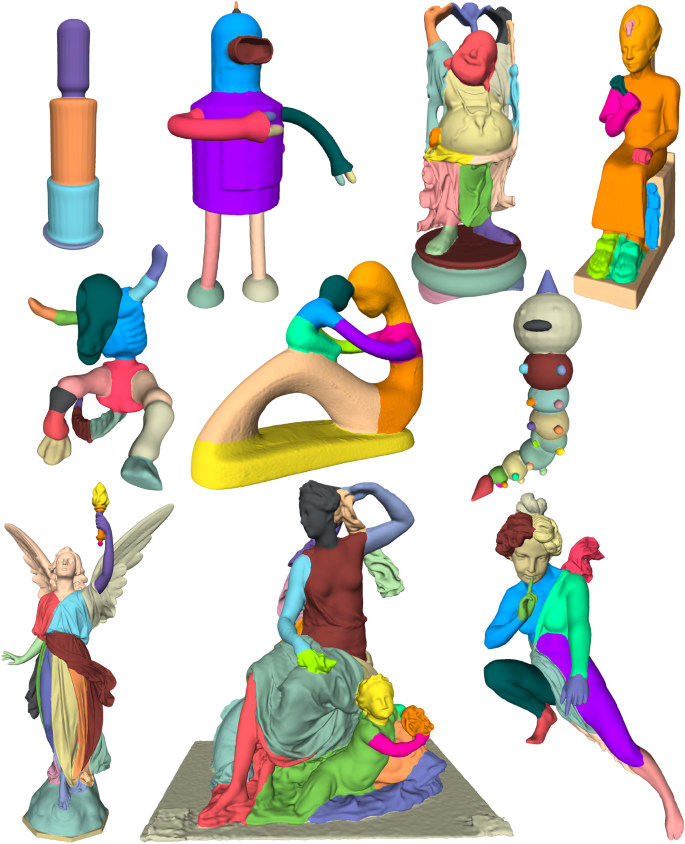
\includegraphics[width=0.8\textwidth]{figures/spectral_partitioning.png}
        \caption{Mesh partitioning from \cite{bao2023spectral}}
    \end{subfigure}\hfill

    \vspace{1cm}
    \begin{subfigure}[t]{0.7\textwidth}
        \centering
        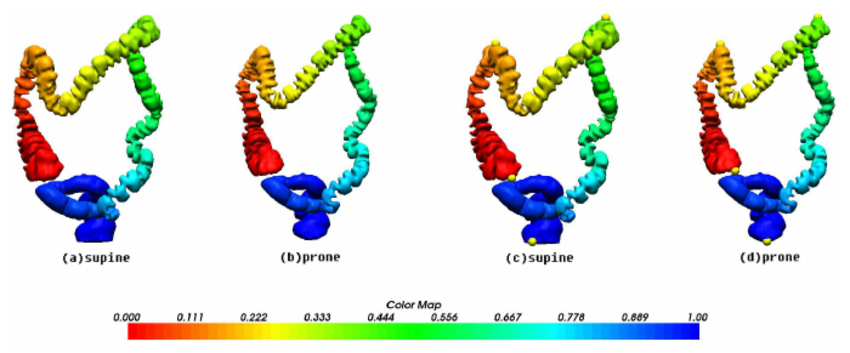
\includegraphics[width=0.7\textwidth]{figures/fielder_vector_colon.png}
        \caption{Mesh partitioning from \cite{10.1007/978-3-642-15705-9_41}}
   \end{subfigure}
    \caption{Examples of spectral partitioning of meshes}
    \label{fig:spectral_part}
\end{figure}

\newpage
\printbibliography

\end{document}
